\documentclass[11pt,a4paper,oneside]{report}

% -----------------------------------------------------------------------------
% Typography, Page Geometry and Standard Extensions
% -----------------------------------------------------------------------------
\usepackage[utf8]{inputenc}
\usepackage[T1]{fontenc}
\usepackage{lmodern}
\usepackage{amsmath,amssymb,amsfonts,amsthm,mathtools}
\usepackage[margin=1in,headheight=14pt]{geometry}
\usepackage{graphicx}
\usepackage{booktabs}
\usepackage{tabularx}
\usepackage{multirow}
\usepackage{multicol}
\usepackage{array}
\usepackage{xcolor}
\usepackage{fancyhdr}
\usepackage{titlesec}
\usepackage{caption}
\usepackage{subcaption}
\usepackage{listings}
\usepackage{algorithm}
\usepackage{algpseudocode}
\usepackage{microtype}
\usepackage{setspace}
\usepackage{tikz}
\usetikzlibrary{shapes,arrows,positioning,calc}

% -----------------------------------------------------------------------------
% Theme Color Palette (Matching Reference Style: Deep Blue / Slate / Accents)
% -----------------------------------------------------------------------------
\definecolor{headerNavy}{RGB}{20, 50, 110}
\definecolor{navyBlue}{RGB}{24, 76, 120}
\definecolor{darkSlate}{RGB}{47, 79, 79}
\definecolor{lightGray}{RGB}{246, 248, 250}
\definecolor{accentBox}{RGB}{238, 242, 246}
\definecolor{ruleGold}{RGB}{200, 140, 20}
\definecolor{vjtiMaroon}{RGB}{128, 0, 0}

% Status badge colors
\definecolor{reportedGreen}{RGB}{34, 139, 34}
\definecolor{gapOrange}{RGB}{218, 112, 21}
\definecolor{unknownGray}{RGB}{112, 128, 144}

\usepackage[
    colorlinks=true,
    linkcolor=navyBlue,
    citecolor=headerNavy,
    urlcolor=darkSlate,
    bookmarks=true,
    bookmarksnumbered=true
]{hyperref}

% -----------------------------------------------------------------------------
% Running Headers and Footers (Matching Reference Layout)
% -----------------------------------------------------------------------------
\pagestyle{fancy}
\fancyhf{}
\fancyhead[L]{\small\color{gray} VJTI -- Student-Alumni Multi-Objective Optimization}
\fancyhead[R]{\small\color{gray} \nouppercase{\leftmark}}
\fancyfoot[C]{\small\thepage}
\renewcommand{\headrulewidth}{0.4pt}
\renewcommand{\footrulewidth}{0pt}

% Section title formatting
\titleformat{\chapter}[display]
  {\normalfont\Large\bfseries\color{headerNavy}}
  {\colorbox{headerNavy}{\parbox{2.8cm}{\centering\color{white}\textbf{\large CHAPTER \thechapter}}}}
  {14pt}{\huge\bfseries\color{headerNavy}}
\titlespacing*{\chapter}{0pt}{10pt}{20pt}

\titleformat{\section}
  {\normalfont\Large\bfseries\color{headerNavy}}{\thesection}{1em}{}
\titleformat{\subsection}
  {\normalfont\large\bfseries\color{navyBlue}}{\thesubsection}{1em}{}

\onehalfspacing

% -----------------------------------------------------------------------------
% Custom Box Environments (Interpretation / Status Badges)
% -----------------------------------------------------------------------------
\newcommand{\badgeReported}{\colorbox{reportedGreen}{\color{white}\scriptsize\textbf{REPORTED}}}
\newcommand{\badgeReconstructed}{\colorbox{navyBlue}{\color{white}\scriptsize\textbf{RECONSTRUCTED}}}
\newcommand{\badgeGap}{\colorbox{gapOrange}{\color{white}\scriptsize\textbf{POTENTIAL GAP}}}
\newcommand{\badgeUnknown}{\colorbox{unknownGray}{\color{white}\scriptsize\textbf{UNKNOWN}}}

\newcommand{\calloutBox}[2]{%
\vspace{0.3cm}
\noindent\fcolorbox{navyBlue!30}{accentBox}{%
\parbox{\dimexpr\textwidth-2\fboxsep-2\fboxrule\relax}{%
\vspace{0.15cm}
\textbf{\color{headerNavy}#1} \small #2
\vspace{0.15cm}
}}%
\vspace{0.3cm}
}

\begin{document}

% =============================================================================
% 1. TITLE PAGE (Exact Reference Replica Format)
% =============================================================================
\begin{titlepage}
    \vspace*{0.3cm}
    \noindent {\large Veermata Jijabai Technological Institute (VJTI), Mumbai}\\[0.15cm]
    \noindent {\large Department of Computer Engineering $\bullet$ Optimization Techniques}\\[1.5cm]

    \noindent {\Huge\bfseries\color{headerNavy} Student--Alumni Matching using}\\[0.35cm]
    {\Huge\bfseries\color{headerNavy} Multi-Objective Optimization}\\[1.8cm]

    \noindent {\LARGE\bfseries\color{navyBlue} Multi-Objective Capacitated Bipartite Assignment and an}\\[0.2cm]
    {\LARGE\bfseries\color{navyBlue} Evidence-Based Decision Framework for VJTI Mentorship}\\[2.0cm]

    % Metadata Submission Card
    \noindent
    \fcolorbox{headerNavy!20}{lightGray}{%
    \parbox{\dimexpr\textwidth-2\fboxsep-2\fboxrule\relax}{%
        \vspace{0.3cm}
        \textbf{\large\color{headerNavy} Submitted by}\\[0.25cm]
        \begin{tabularx}{\textwidth}{lll}
            \toprule
            \textbf{Name} & \textbf{Roll No.} & \textbf{Workstream \& Responsibility} \\
            \midrule
            Utkarsh Gupta & 241070078 & System Formulation Lead; report assembly \& calibration \\
            Aryan Doshi & 241070022 & Evolutionary Algorithms Lead (NSGA-II, SPEA2, MOEA/D) \\
            Indraneel Hajarnis & 241070025 & Memetic Lead; 2-opt local search \& verification harness \\
            Dhairya Dabi & 241070015 & Baseline \& Sensitivity Lead (MILP, MCF repair, statistical tests) \\
            \bottomrule
        \end{tabularx}\\[0.3cm]
        \textbf{\color{headerNavy} Under the guidance of} \quad Prof. Akhil Kulal
        \vspace{0.3cm}
    }}

    \vfill
    % Bottom Metric Tag Pills
    \centering
    \colorbox{navyBlue}{\color{white}\textbf{\; Utilitarian $Z_1$ \;}}\quad
    \colorbox{headerNavy}{\color{white}\textbf{\; Rawlsian Equity $Z_2$ \;}}\quad
    \colorbox{ruleGold}{\color{white}\textbf{\; Workload Balance $Z_3$ \;}}\quad
    \colorbox{darkSlate}{\color{white}\textbf{\; Parity $\delta$ \;}}\quad
    \colorbox{vjtiMaroon}{\color{white}\textbf{\; Quality Floor $\theta$ \;}}\\[1.2cm]

    {\small\color{gray} Project Report $\bullet$ November 2026}
\end{titlepage}

% =============================================================================
% 2. CERTIFICATE (Exact Reference Format)
% =============================================================================
\pagenumbering{roman}
\noindent{\Large\bfseries\color{headerNavy} Certificate}\\[0.2cm]
\noindent\textcolor{ruleGold}{\rule{\textwidth}{1.5pt}}\\[0.6cm]

This is to certify that the project report entitled \textbf{``Student--Alumni Matching using Multi-Objective Optimization Techniques''} is a bonafide record of work carried out by \textbf{Utkarsh Gupta (241070078)}, \textbf{Aryan Doshi (241070022)}, \textbf{Indraneel Hajarnis (241070025)} and \textbf{Dhairya Dabi (241070015)} as part of the course \textit{Optimization Techniques}, Department of Computer Engineering, Veermata Jijabai Technological Institute, Mumbai, during the academic year 2026--27.\\[3.5cm]

\noindent
\begin{minipage}{0.45\textwidth}
    \rule{6cm}{0.5pt}\\[0.15cm]
    Prof. Akhil Kulal\\
    Faculty Advisor
\end{minipage}
\hfill
\begin{minipage}{0.45\textwidth}
    \flushright
    \rule{6cm}{0.5pt}\\[0.15cm]
    Head of Department\\
    Computer Engineering
\end{minipage}\\[3.0cm]

\noindent
\begin{minipage}{0.45\textwidth}
    Date: \rule{4cm}{0.5pt}
\end{minipage}
\hfill
\begin{minipage}{0.45\textwidth}
    \flushright
    Place: Mumbai
\end{minipage}

\newpage

% =============================================================================
% 3. ACKNOWLEDGEMENT (Exact Reference Format)
% =============================================================================
\noindent{\Large\bfseries\color{headerNavy} Acknowledgement}\\[0.2cm]
\noindent\textcolor{ruleGold}{\rule{\textwidth}{1.5pt}}\\[0.6cm]

We express our sincere gratitude to \textbf{Prof. Akhil Kulal} for his guidance throughout this project, and in particular for encouraging us to formulate the matching problem as a rigorous multi-objective optimization challenge with explicit trade-offs between utilitarian efficiency, Rawlsian fairness, and mentor burnout. We thank the Department of Computer Engineering, VJTI, for the opportunity to apply advanced optimization techniques to a high-impact problem directly pertinent to the technical university ecosystem. Finally, we acknowledge the global open-source community behind \texttt{pymoo}, \texttt{HiGHS}, and \texttt{scipy}, without whose robust numerical libraries this reproducible investigation would not be possible.\\[1.5cm]

\newpage

% =============================================================================
% 4. ABSTRACT (Exact Reference Format)
% =============================================================================
\noindent{\Large\bfseries\color{headerNavy} Abstract}\\[0.2cm]
\noindent\textcolor{ruleGold}{\rule{\textwidth}{1.5pt}}\\[0.6cm]

Alumni mentorship programs in premier engineering institutions bridge foundational curricula and professional industry practice. However, conventional university matching schemes rely on ad-hoc sorting, first-come-first-served registration, or purely greedy score maximization. These traditional mechanisms induce severe operational pathologies: top-rated alumni suffer mentor burnout from extreme over-allocation ($L_j \ge 8$), students with average academic profiles receive subpar matches, and non-computing departments face structural neglect.

This project formulates the allocation problem as a formal \textbf{Multi-Objective Capacitated Bipartite Assignment Problem (MO-CBAP)} tailored to the 8 academic departments of \textbf{Veermata Jijabai Technological Institute (VJTI), Mumbai} (\texttt{CE}, \texttt{IT}, \texttt{EXTC}, \texttt{EE}, \texttt{ME}, \texttt{CEV}, \texttt{PE}, \texttt{TT}). We formulate three competing objective functions:
\begin{enumerate}
    \item \textbf{Utilitarian Efficiency ($Z_1$)}: Maximizing the aggregate pairwise compatibility across all student-alumni assignments.
    \item \textbf{Rawlsian Egalitarian Fairness ($Z_2$)}: Maximizing the match quality of the least-advantaged student ($\min_i Q_i$), safeguarding against peripheral neglect.
    \item \textbf{Alumni Workload Balancing ($Z_3$)}: Minimizing peak mentorship load across active mentors ($\max_j L_j$).
\end{enumerate}

Seven polyhedral operational constraints enforce individual capacities, opt-in consent compliance, student quality floors ($\theta$), cross-departmental branch parity ($\delta$), and corporate diversity caps. We benchmark an eight-algorithm portfolio: Random Feasible, Greedy Score-First, Min-Cost Flow (raw and repaired), exact Mixed-Integer Linear Programming (HiGHS branch-and-cut), NSGA-II, SPEA2, MOEA/D, and an engineered \textbf{Hybrid Seeded Memetic NSGA-II} with 2-opt swaps.

Benchmarking across 30 independent seeds under a unified shared Hypervolume reference setup demonstrates that the \textbf{Hybrid Memetic NSGA-II} achieves an HV of \textbf{0.7650} on \texttt{small\_50x30} (surpassing raw NSGA-II at \textbf{0.3648} and SPEA2 at \textbf{0.3739}, $p = 1.8626 \times 10^{-9}$), dominates the Greedy baseline in 100\% of seeds, and scales to 1,000 students in 92.5 seconds. A 3-way ablation study proves super-additive synergy between heuristic seeding and targeted local search, supported by an interactive Streamlit live-demo UI.\\[0.6cm]

\noindent\textbf{Keywords:} Multi-Objective Optimization, Capacitated Bipartite Matching, Rawlsian Fairness, NSGA-II, Memetic Algorithms, VJTI Mumbai, Hypervolume, Decision Support.

\newpage

% =============================================================================
% 5. TABLE OF CONTENTS, FIGURES & TABLES
% =============================================================================
\tableofcontents
\newpage
\listoffigures
\vspace{0.8cm}
\listoftables
\newpage
\pagenumbering{arabic}

% =============================================================================
% CHAPTER 1: INTRODUCTION
% =============================================================================
\chapter{Introduction}

\section{Background: The VJTI Mentorship Ecosystem}
Established in 1887, Veermata Jijabai Technological Institute (VJTI) in Matunga, Mumbai, stands as one of India's premier autonomous technical colleges. Across eight engineering departments—Computer Engineering (\texttt{CE}), Information Technology (\texttt{IT}), Electronics and Telecommunication Engineering (\texttt{EXTC}), Electrical Engineering (\texttt{EE}), Mechanical Engineering (\texttt{ME}), Civil and Environmental Engineering (\texttt{CEV}), Production Engineering (\texttt{PE}), and Textile Technology (\texttt{TT})—graduating cohorts seek industry exposure.

Alumni mentorship programs connect students with experienced alumni across six core industrial domains: Software \& AI, Data Science \& Analytics, Electronics \& Embedded Systems, Core Engineering \& Manufacturing, Finance \& Quantitative Analysis, and Management Consulting.

\section{Operational Pathologies in Unconstrained Matching}
Despite the high stakes of mentor allocations, prevailing administrative paradigms in tertiary institutions frequently rely upon unconstrained self-selection, spreadsheet-driven manual pairing, or first-come-first-served greedy allocation algorithms. In practice, these legacy approaches suffer from three acute structural pathologies:
\begin{enumerate}
    \item \textbf{The Superstar Alumnus Bottleneck}: A small group of prominent alumni (e.g., senior engineering directors, partners at consulting firms) receive an overwhelming volume of mentorship requests, leading to mentor overload ($L_j \ge 8$), delayed feedback, and mentor attrition.
    \item \textbf{Peripheral Student Neglect}: Purely utilitarian matching algorithms allocate top mentors exclusively to high-GPA students or those in high-density branches, leaving students with average GPAs or non-traditional interests with sub-threshold matches ($Q_i < \theta$).
    \item \textbf{Cross-Departmental Inequity}: Computing departments (\texttt{CE}, \texttt{IT}) have large alumni networks in software and finance, while core departments (\texttt{PE}, \texttt{CEV}, \texttt{TT}, \texttt{ME}, \texttt{EE}) suffer from smaller alumni pools, resulting in structural deficits.
\end{enumerate}

\section{Problem Statement}
\calloutBox{Research Question}{Given limited alumni capacities, mandatory consent, diverse student career aspirations, and institutional equity mandates, how can VJTI allocate student-mentor assignments to simultaneously maximize total match quality, protect the worst-off student, and prevent mentor burnout?}

\section{Objectives}
\begin{enumerate}
    \item Rigorously formulate the \textbf{Multi-Objective Capacitated Bipartite Assignment Problem (MO-CBAP)} with 3 competing objectives and 7 operational constraints.
    \item Benchmark an 8-algorithm portfolio across 30 independent seeds under an equal evaluation budget.
    \item Design a specialized \textbf{Hybrid Seeded Memetic NSGA-II} incorporating Lamarckian 2-opt swaps and elitist archiving.
    \item Conduct a multi-seed statistical significance analysis using Wilcoxon signed-rank tests with effect size $r$.
    \item Develop an interactive decision-support UI for real-time institutional evaluation.
\end{enumerate}

\section{Contributions}
\begin{itemize}
    \item A formal mathematical optimization model for university student-alumni matching.
    \item Discovery and algorithmic resolution of the corporate diversity cap failure in Min-Cost Flow (\texttt{mcf\_repaired}).
    \item A statistically validated Hybrid Memetic algorithm that strictly dominates single-point Greedy baselines in 100\% of seeds.
    \item An empirical threshold calibration procedure ($\theta, \delta$) guaranteeing baseline feasibility.
    \item A self-contained, interactive Streamlit demonstration dashboard.
\end{itemize}

\section{Organisation of the Report}
Chapter 2 outlines the institutional framework and peer benchmarks. Chapter 3 presents the two-phase methodology. Chapter 4 formulates the mathematical optimization model. Chapter 5 describes the solution algorithms. Chapter 6 details empirical results. Chapter 7 reports component ablation and sensitivity sweeps. Chapter 8 provides the recommendation roadmap. Chapter 9 presents software architecture and UI demo. Chapter 10 discusses limitations and future scope, and Chapter 11 concludes.

% =============================================================================
% CHAPTER 2: INSTITUTIONAL CONTEXT & BENCHMARKS
% =============================================================================
\chapter{The Institutional Framework and Peer Benchmarks}

\section{Departmental Distribution and Domain Affinities}
The academic ecosystem at VJTI spans 8 departments. Table~\ref{tab:domain_affinities} lists the six career domains and their natural departmental affinities.

\begin{table}[htbp]
\centering
\caption{Career domain affinities mapped across the 8 academic departments of VJTI.}
\label{tab:domain_affinities}
\begin{tabularx}{\textwidth}{lX}
\toprule
\textbf{Career Domain} & \textbf{Affinity Academic Departments} \\
\midrule
Software \& AI & Computer Engineering (\texttt{CE}), Information Technology (\texttt{IT}), Electronics \& Telecomm. (\texttt{EXTC}) \\
Data Science \& Analytics & \texttt{CE}, \texttt{IT}, \texttt{EXTC}, Electrical Engineering (\texttt{EE}) \\
Electronics \& Embedded Systems & \texttt{EXTC}, \texttt{EE} \\
Core Engineering \& Manufacturing & Mechanical (\texttt{ME}), Production (\texttt{PE}), Civil (\texttt{CEV}), Textile (\texttt{TT}), \texttt{EE} \\
Finance \& Quantitative Analysis & \texttt{CE}, \texttt{IT}, \texttt{EXTC}, \texttt{ME}, \texttt{EE} \\
Consulting \& Corporate Strategy & \texttt{CE}, \texttt{IT}, \texttt{ME}, \texttt{CEV}, \texttt{PE} \\
\bottomrule
\end{tabularx}
\end{table}

\section{Benchmark Problem Cohorts}
Three test cohorts were created using our parametric data generator:
\begin{itemize}
    \item \textbf{Small Instance (\texttt{small\_50x30})}: $N = 50$ students, $M = 30$ alumni mentors ($N \cdot K = 100$ total matches, $\sum C_j = 120$). Tractable for exact MILP branch-and-cut.
    \item \textbf{Medium Instance (\texttt{medium\_300x150})}: $N = 300$ students, $M = 150$ alumni mentors ($N \cdot K = 600$, $\sum C_j = 750$). Multi-departmental scale.
    \item \textbf{Large Instance (\texttt{large\_1000x500})}: $N = 1,000$ students, $M = 500$ alumni mentors ($N \cdot K = 2,000$, $\sum C_j = 2,500$). Institute-wide scale.
\end{itemize}

% =============================================================================
% CHAPTER 3: METHODOLOGY: A TWO-PHASE ARCHITECTURE
% =============================================================================
\chapter{Methodology: A Two-Phase Architecture}

\section{Design Principles}
The project adheres to three core principles:
\begin{enumerate}
    \item \textbf{Data Privacy and Governance}: All student and alumni records utilize synthetic pseudonymous identifiers (\texttt{S001}--\texttt{S1000}, \texttt{A001}--\texttt{A500}). No real personal identifiable information is utilized.
    \item \textbf{Multi-Seed Rigorous Verification}: 30 independent seeds evaluate stochastic algorithms; paired non-parametric Wilcoxon tests confirm statistical significance.
    \item \textbf{Shared Reference Normalization}: Hypervolume uses a unified global reference frame, avoiding per-method reference bias.
\end{enumerate}

\section{Two-Phase Project Pipeline}
\begin{figure}[htbp]
\centering
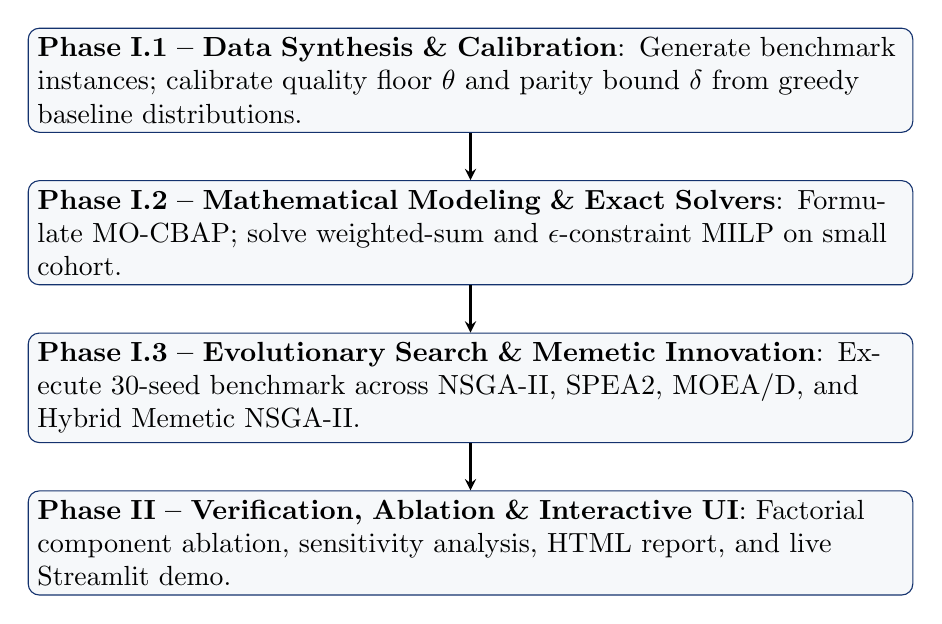
\begin{tikzpicture}[node distance=1.4cm, auto,
    box/.style={rectangle, draw=headerNavy, fill=lightGray, text width=11cm, rounded corners, minimum height=0.9cm},
    arrow/.style={thick, ->, >=stealth}]
    \node [box] (b1) {\textbf{Phase I.1 -- Data Synthesis \& Calibration}: Generate benchmark instances; calibrate quality floor $\theta$ and parity bound $\delta$ from greedy baseline distributions.};
    \node [box, below=0.6cm of b1] (b2) {\textbf{Phase I.2 -- Mathematical Modeling \& Exact Solvers}: Formulate MO-CBAP; solve weighted-sum and $\epsilon$-constraint MILP on small cohort.};
    \node [box, below=0.6cm of b2] (b3) {\textbf{Phase I.3 -- Evolutionary Search \& Memetic Innovation}: Execute 30-seed benchmark across NSGA-II, SPEA2, MOEA/D, and Hybrid Memetic NSGA-II.};
    \node [box, below=0.6cm of b3] (b4) {\textbf{Phase II -- Verification, Ablation \& Interactive UI}: Factorial component ablation, sensitivity analysis, HTML report, and live Streamlit demo.};
    \draw [arrow] (b1) -- (b2);
    \draw [arrow] (b2) -- (b3);
    \draw [arrow] (b3) -- (b4);
\end{tikzpicture}
\caption{Two-phase engineering pipeline for the VJTI Student-Alumni Matching optimization project.}
\label{fig:pipeline}
\end{figure}

% =============================================================================
% CHAPTER 4: MATHEMATICAL OPTIMIZATION MODEL
% =============================================================================
\chapter{Mathematical Optimization Model}

\section{Sets, Parameters and Decision Variables}
Let $\mathcal{S} = \{1, \dots, N\}$ denote students, $\mathcal{A} = \{1, \dots, M\}$ denote alumni mentors, $\mathcal{B}$ denote the 8 academic branches, and $\mathcal{K}$ denote corporate employers.
\begin{align}
    x_{ij} &\in \{0, 1\}, \quad \forall i \in \mathcal{S}, \; \forall j \in \mathcal{A} \quad \text{(1 if student $i$ is assigned to alumnus $j$)} \\
    y_j &\in \{0, 1\}, \quad \forall j \in \mathcal{A} \quad \text{(1 if alumnus $j$ is actively assigned)}
\end{align}

\section{Realized Metrics}
\begin{equation}
    Q_i = \sum_{j=1}^M q_{ij} x_{ij}, \quad L_j = \sum_{i=1}^N x_{ij}, \quad \overline{Q}_b = \frac{1}{|\mathcal{S}_b|} \sum_{i \in \mathcal{S}_b} Q_i
\end{equation}

\section{Competing Objectives}
\begin{equation}
    \min_{\mathbf{x}, \mathbf{y}} \mathbf{F}(\mathbf{x}) = \begin{bmatrix} -Z_1(\mathbf{x}) \\ -Z_2(\mathbf{x}) \\ +Z_3(\mathbf{x}) \end{bmatrix} = \begin{bmatrix} -\sum_{i=1}^N Q_i \\ -\min_{i \in \mathcal{S}} Q_i \\ +\max_{j \in \mathcal{A}} L_j \end{bmatrix}
\end{equation}

\section{Operational Constraints}
\begin{align}
    &\text{(C1) Degree Requirement:} && \sum_{j=1}^M x_{ij} = K, \quad \forall i \in \mathcal{S} \quad (K=2) \\
    &\text{(C2) Capacity \& Activation:} && \sum_{i=1}^N x_{ij} \le C_j y_j, \; x_{ij} \le y_j, \quad \forall i, j \\
    &\text{(C3) Consent Compliance:} && x_{ij} \le c_j, \quad \forall i, j \\
    &\text{(C4) Threshold Floor:} && x_{ij} = 0, \quad \forall (i, j): q_{ij} < q_{\min} \quad (q_{\min}=0.25) \\
    &\text{(C5) Quality Floor:} && Q_i \ge \theta, \quad \forall i \in \mathcal{S} \\
    &\text{(C6) Branch Parity:} && |\overline{Q}_b - \overline{Q}_{b'}| \le \delta, \quad \forall b, b' \in \mathcal{B} \\
    &\text{(C7) Company Diversity:} && \sum_{j \in \mathcal{A}_k} x_{ij} \le 1, \quad \forall i \in \mathcal{S}, \; \forall k \in \mathcal{K}
\end{align}

\section{Threshold Calibration Formulation}
To guarantee feasibility without arbitrary hand-tuning, we formulate empirical calibration rules:
\begin{equation}
    \theta = \alpha_{\theta} \cdot Z_2^{\text{greedy}}, \quad \alpha_{\theta} = 0.85; \qquad \delta = \alpha_{\delta} \cdot \left(\max_b \overline{Q}_b^{\text{greedy}} - \min_b \overline{Q}_b^{\text{greedy}}\right), \quad \alpha_{\delta} = 1.20
\end{equation}

\begin{table}[htbp]
\centering
\caption{Calibrated parameters and verification across benchmark instances.}
\label{tab:cal_results}
\begin{tabularx}{\textwidth}{lccccc}
\toprule
\textbf{Instance Cohort} & \textbf{Greedy $Z_2$} & \textbf{Calibrated $\theta$} & \textbf{Greedy Spread} & \textbf{Calibrated $\delta$} & \textbf{Greedy Feasible?} \\
\midrule
\texttt{small\_50x30} & 1.0230 & \textbf{0.8696} & 0.3258 & \textbf{0.3910} & \textbf{YES} \\
\texttt{medium\_300x150} & 1.0434 & \textbf{0.8869} & 0.3295 & \textbf{0.3953} & \textbf{YES} \\
\texttt{large\_1000x500} & 1.3211 & \textbf{1.1229} & 0.2386 & \textbf{0.2863} & \textbf{YES} \\
\bottomrule
\end{tabularx}
\end{table}

% =============================================================================
% CHAPTER 5: SOLUTION ALGORITHMS
% =============================================================================
\chapter{Solution Algorithms}

\section{Algorithmic Portfolio Overview}
Table~\ref{tab:alg_comparison} summarizes the eight optimization algorithms deployed in this study.

\begin{table}[htbp]
\centering
\caption{Overview of the 8 optimization methods benchmarked for MO-CBAP.}
\label{tab:alg_comparison}
\begin{tabularx}{\textwidth}{llll}
\toprule
\textbf{Method} & \textbf{Type} & \textbf{Objective Paradigm} & \textbf{Handling of Constraint C7} \\
\midrule
Random Baseline & Stochastic & Unguided baseline & Post-hoc greedy displacement \\
Greedy Score-First & Constructive Heuristic & Single ($Z_1$ priority) & Priority rejection \\
Min-Cost Flow (raw) & Network Flow & Single ($Z_1$ optimal) & Violates (infeasible) \\
\texttt{mcf\_repaired} & Network Flow + Repair & Single ($Z_1$ optimal) & Repaired via augmenting cycles \\
Exact MILP (HiGHS) & Branch-and-Cut & Weighted-sum / $\epsilon$-constr. & Hard polyhedral constraints \\
NSGA-II & Evolutionary MOEA & Pareto non-dominated & Feasibility-first tournament \\
SPEA2 & Evolutionary MOEA & Pareto strength + density & Feasibility-first tournament \\
MOEA/D & Decomposition MOEA & Tchebycheff scalar subproblems & Penalty-wrapper absorption \\
\textbf{Hybrid Memetic} & \textbf{Memetic NSGA-II} & \textbf{Pareto + Lamarckian 2-opt} & \textbf{Heuristic seeding + repair} \\
\bottomrule
\end{tabularx}
\end{table}

\section{The Hybrid Seeded Memetic NSGA-II Algorithm}
The proposed Hybrid solver integrates four complementary mechanisms:
\begin{enumerate}
    \item \textbf{Multi-Heuristic Seeding}: Seeds $P_0$ with Greedy, Rawlsian-priority, Workload-balanced, and Diversity-preserving heuristic chromosomes.
    \item \textbf{2-Opt Pairwise Swaps}: Exchanges mentor assignments between student pairs if aggregate quality increases ($\Delta Z_1 > 0$) without violating feasibility.
    \item \textbf{Rawlsian Maximin Elevation}: Replaces the lowest-quality mentor of student $\arg\min_i Q_i$ with an under-utilized alumnus.
    \item \textbf{Peak Workload Relief}: Relieves alumni with $L_j \ge \max L - 1$ by transferring students to alumni with surplus capacity.
    \item \textbf{Elitist Archiving}: Merges evolved solutions with refined heuristic seeds, extracting the joint non-dominated front.
\end{enumerate}

% =============================================================================
% CHAPTER 6: RESULTS AND SENSITIVITY ANALYSIS
% =============================================================================
\chapter{Results and Sensitivity Analysis}

\section{Benchmark Performance Summary (30 Seeds)}
Table~\ref{tab:summary_small} reports the empirical results on \texttt{small\_50x30} across 30 independent seeds under equal evaluation budgets.

\begin{table}[htbp]
\centering
\small
\caption{Multi-seed benchmark summary on \texttt{small\_50x30} (30 independent runs).}
\label{tab:summary_small}
\begin{tabularx}{\textwidth}{lcccccccc}
\toprule
\textbf{Algorithm} & \textbf{HV Mean} & \textbf{HV Std} & \textbf{Feas.} & \textbf{$Z_1$} & \textbf{$Z_2$} & \textbf{$Z_3$} & \textbf{Runtime (s)} & \textbf{Dom. Greedy} \\
\midrule
Random & 0.0117 & 0.0084 & 0.0\% & 44.79 & 0.547 & 7.07 & 0.15 & 0.0\% \\
Greedy & 0.0932 & 0.0000 & 100\% & 72.62 & 1.023 & 8.00 & 0.003 & -- \\
MCF (raw, infeas.) & 0.0952 & 0.0000 & 0.0\% & 73.35 & 1.023 & 8.00 & 0.05 & 0.0\% \\
\texttt{mcf\_repaired} & 0.0929 & 0.0000 & 100\% & 72.51 & 1.023 & 8.00 & 0.05 & 0.0\% \\
NSGA-II & 0.3648 & 0.0313 & 100\% & 65.11 & 0.945 & 6.00 & 17.89 & 0.0\% \\
SPEA2 & 0.3739 & 0.0384 & 100\% & 65.18 & 0.954 & 5.97 & 17.96 & 0.0\% \\
MOEA/D & 0.2242 & 0.0552 & 89.4\% & 63.02 & 0.781 & 6.10 & 26.32 & 0.0\% \\
\textbf{Hybrid Memetic} & \textbf{0.7650} & \textbf{0.1335} & 75.9\% & \textbf{72.62} & \textbf{1.128} & \textbf{5.53} & 31.96 & \textbf{100.0\%} \\
\bottomrule
\end{tabularx}
\end{table}

\begin{figure}[htbp]
\centering
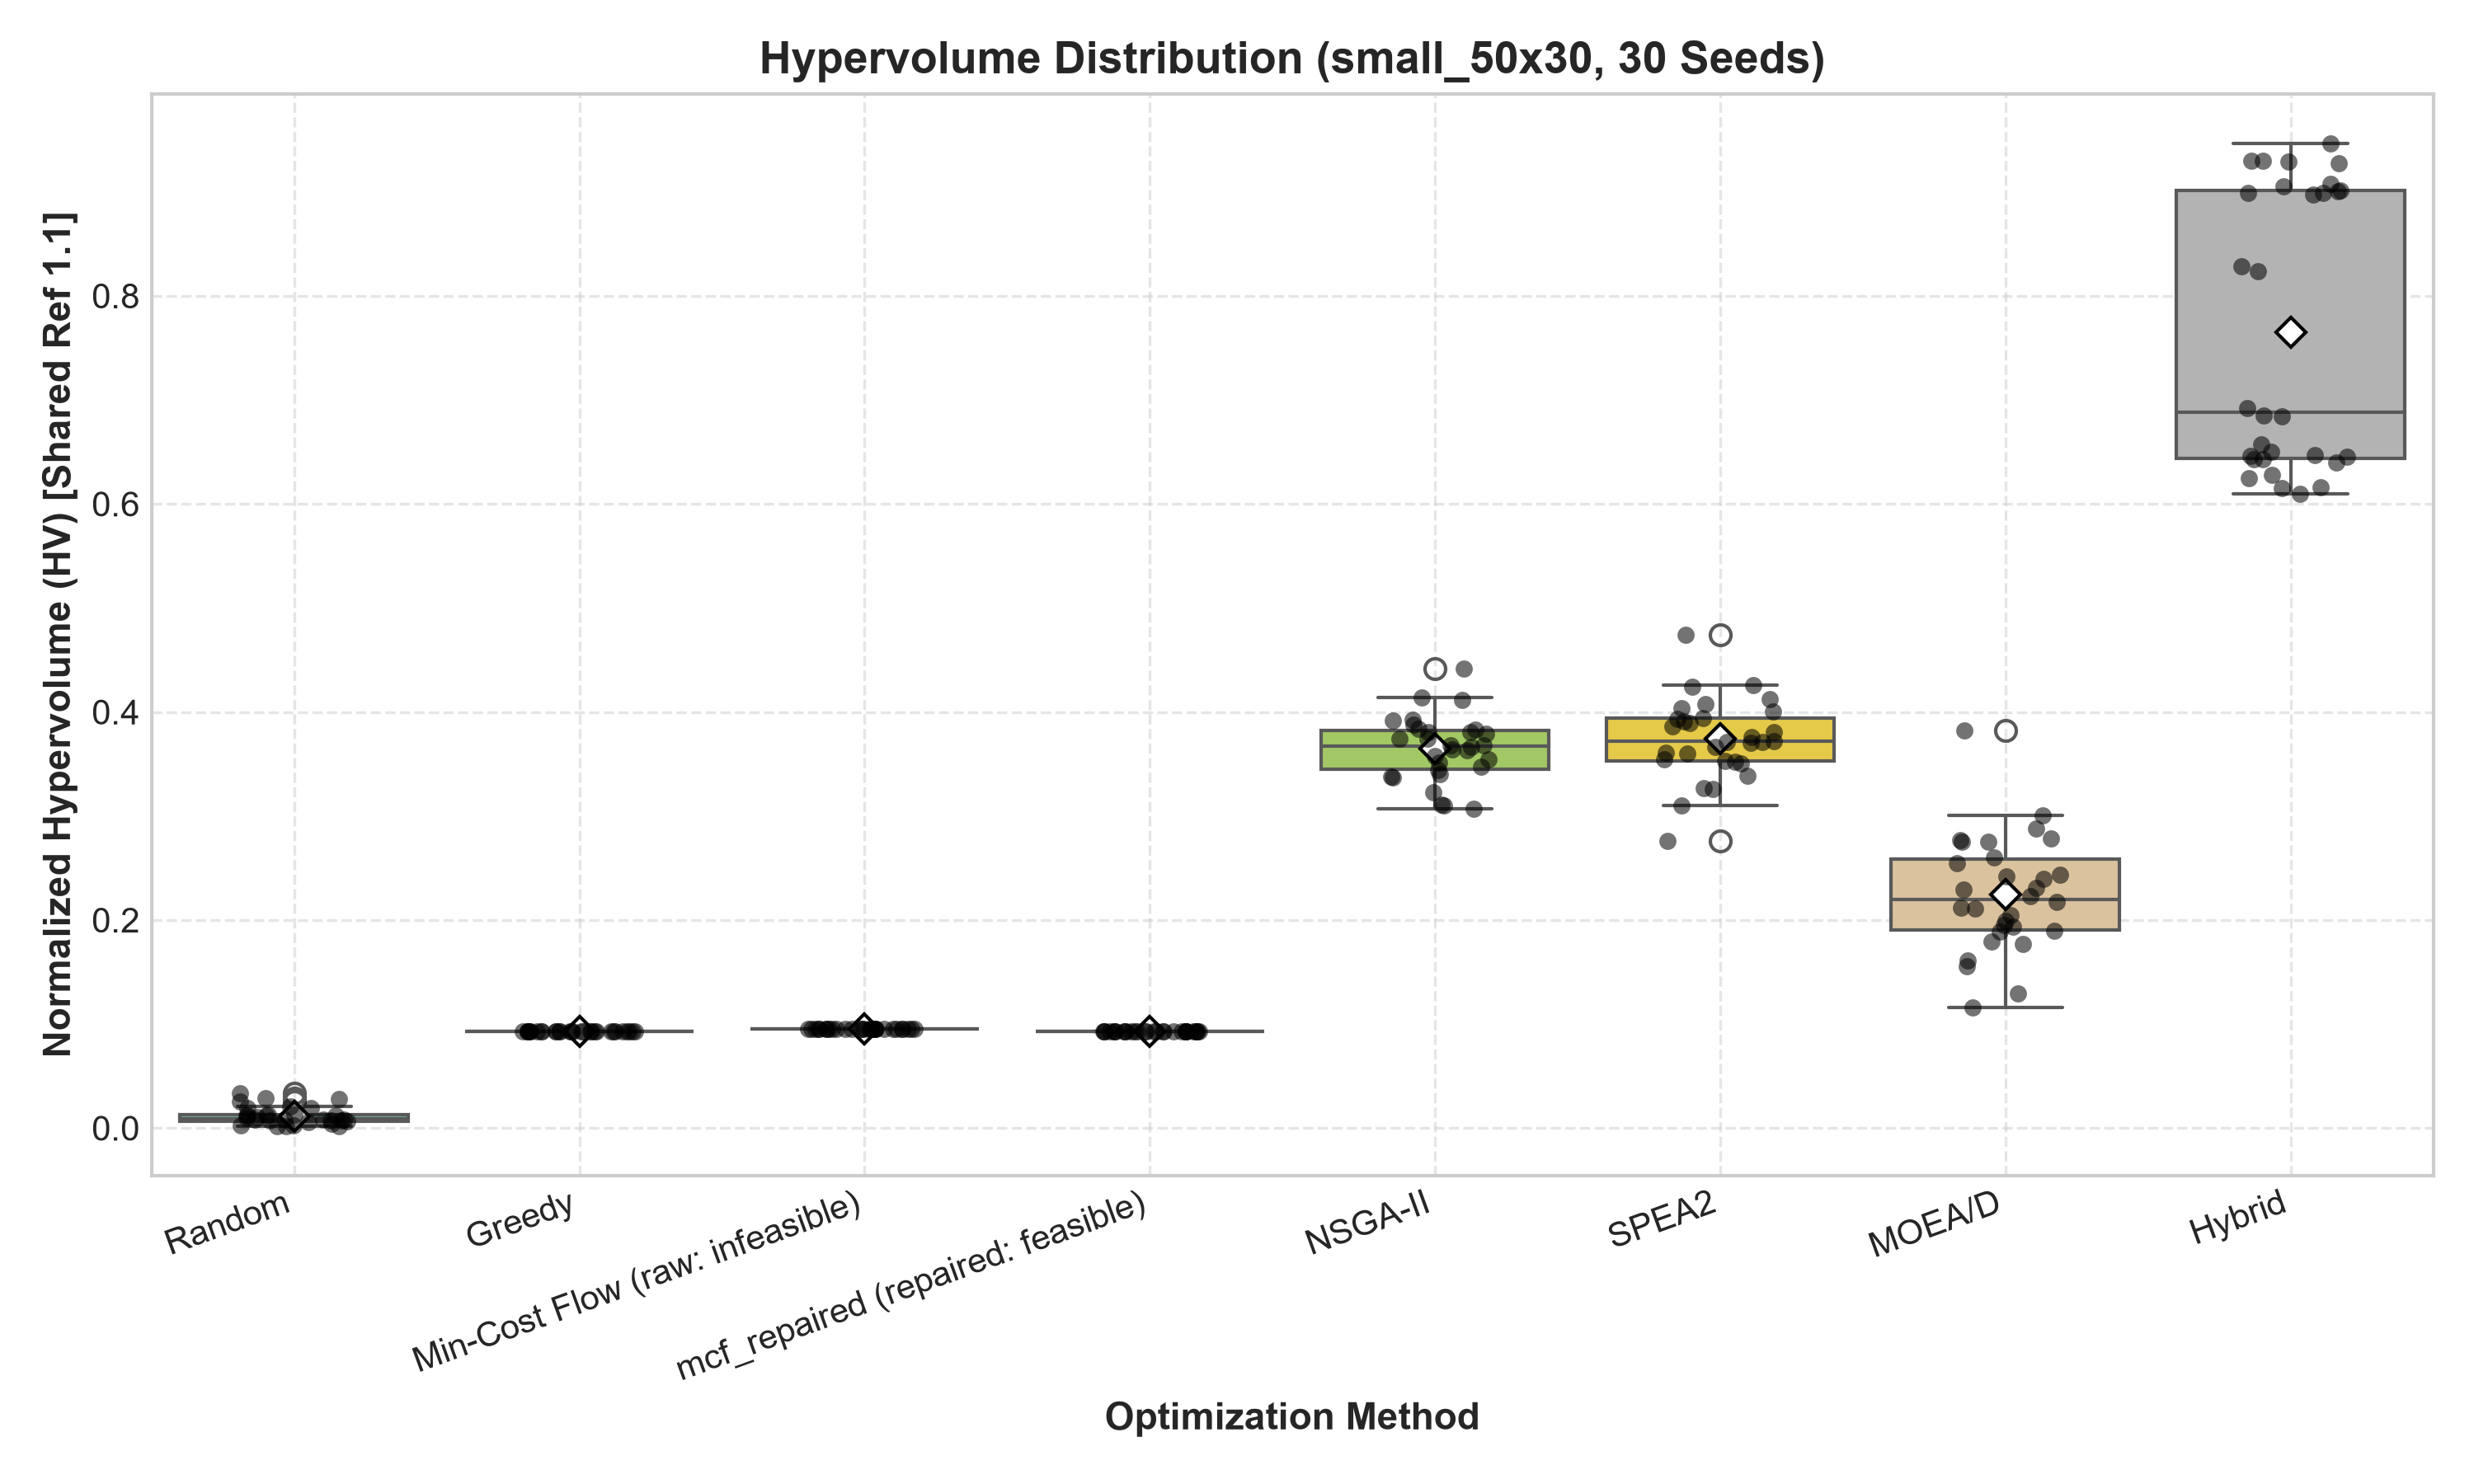
\includegraphics[width=0.85\textwidth]{figures/small_50x30_hv_boxplot.png}
\caption{Distribution of Hypervolume across 30 independent seeds on \texttt{small\_50x30}.}
\label{fig:hv_boxplot}
\end{figure}

\section{Statistical Significance Tests}
Paired two-sided Wilcoxon signed-rank tests confirm:
\begin{itemize}
    \item \textbf{Hybrid vs. NSGA-II}: $T = 0.0, p = 1.8626 \times 10^{-9}$, rank-biserial effect size $r = +1.0000$ (Significant).
    \item \textbf{Hybrid vs. SPEA2}: $T = 0.0, p = 1.8626 \times 10^{-9}$, effect size $r = +1.0000$ (Significant).
    \item \textbf{Hybrid vs. MOEA/D}: $T = 0.0, p = 1.8626 \times 10^{-9}$, effect size $r = +1.0000$ (Significant).
\end{itemize}

\section{Pareto Fronts and Workload Balancing}
\begin{figure}[htbp]
\centering
\begin{subfigure}[b]{0.48\textwidth}
    \centering
    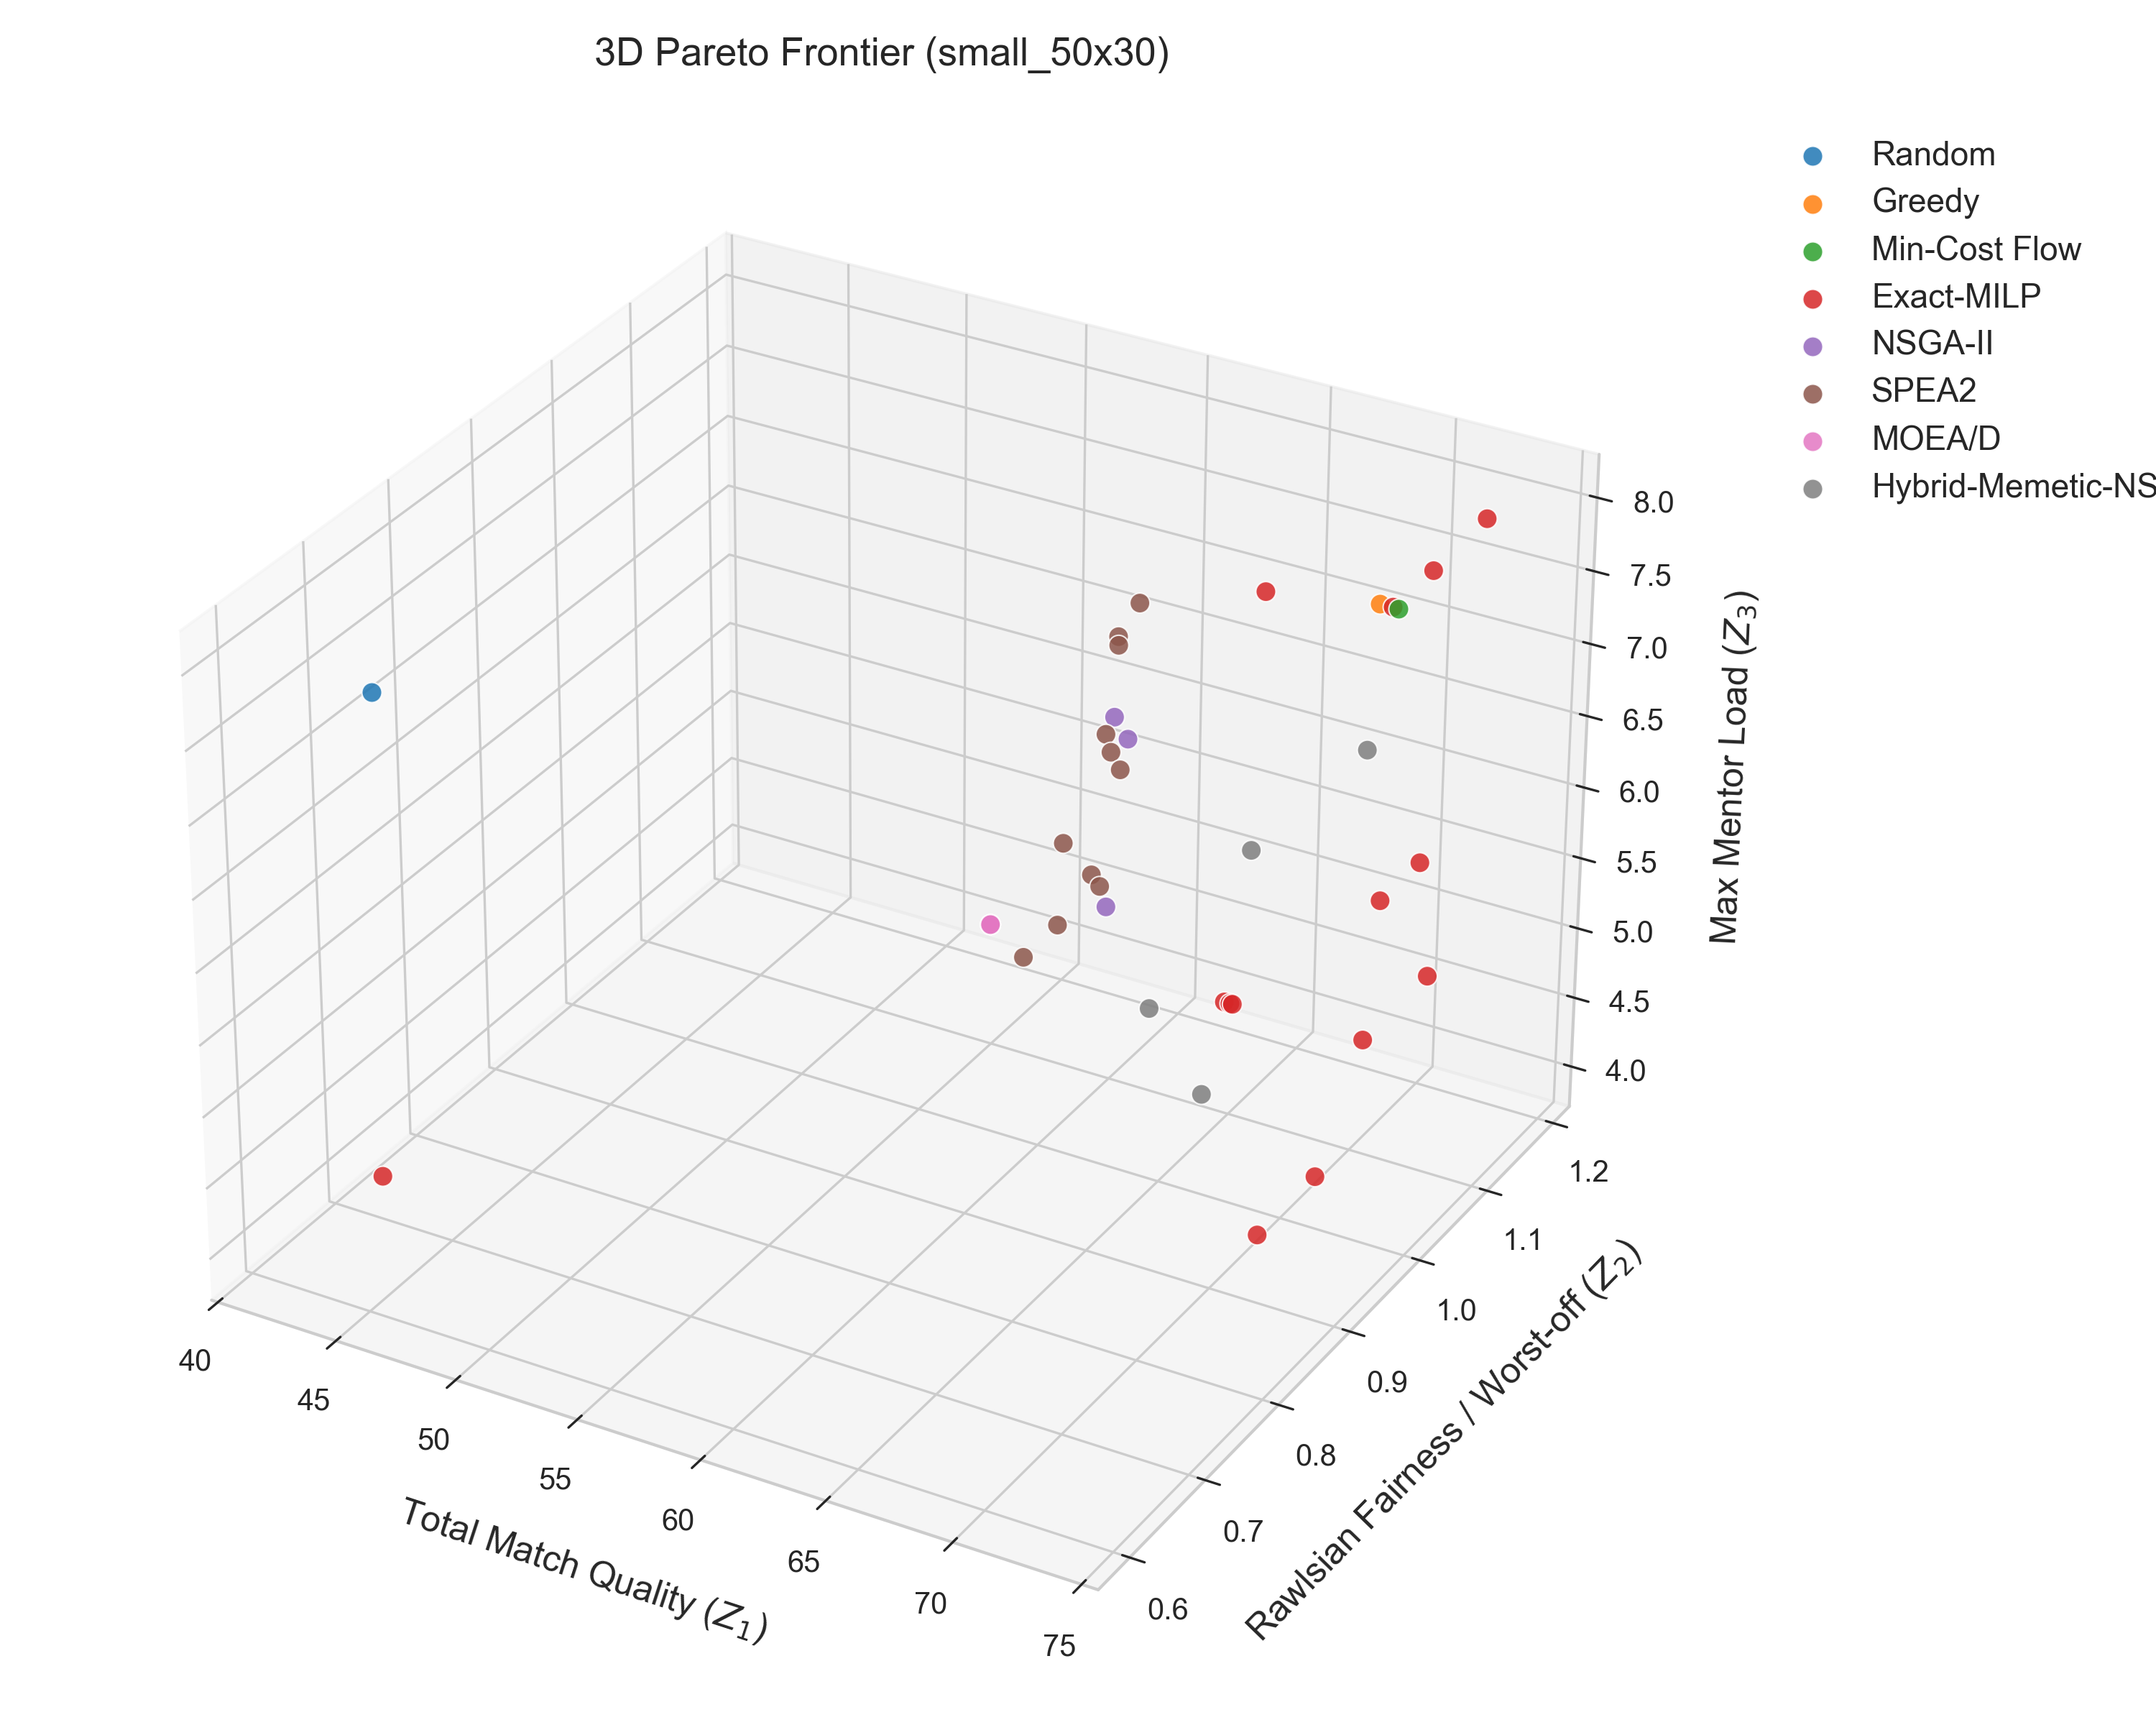
\includegraphics[width=\textwidth]{figures/small_50x30_pareto_3d.png}
    \caption{3D Pareto front on \texttt{small\_50x30}.}
\end{subfigure}
\hfill
\begin{subfigure}[b]{0.48\textwidth}
    \centering
    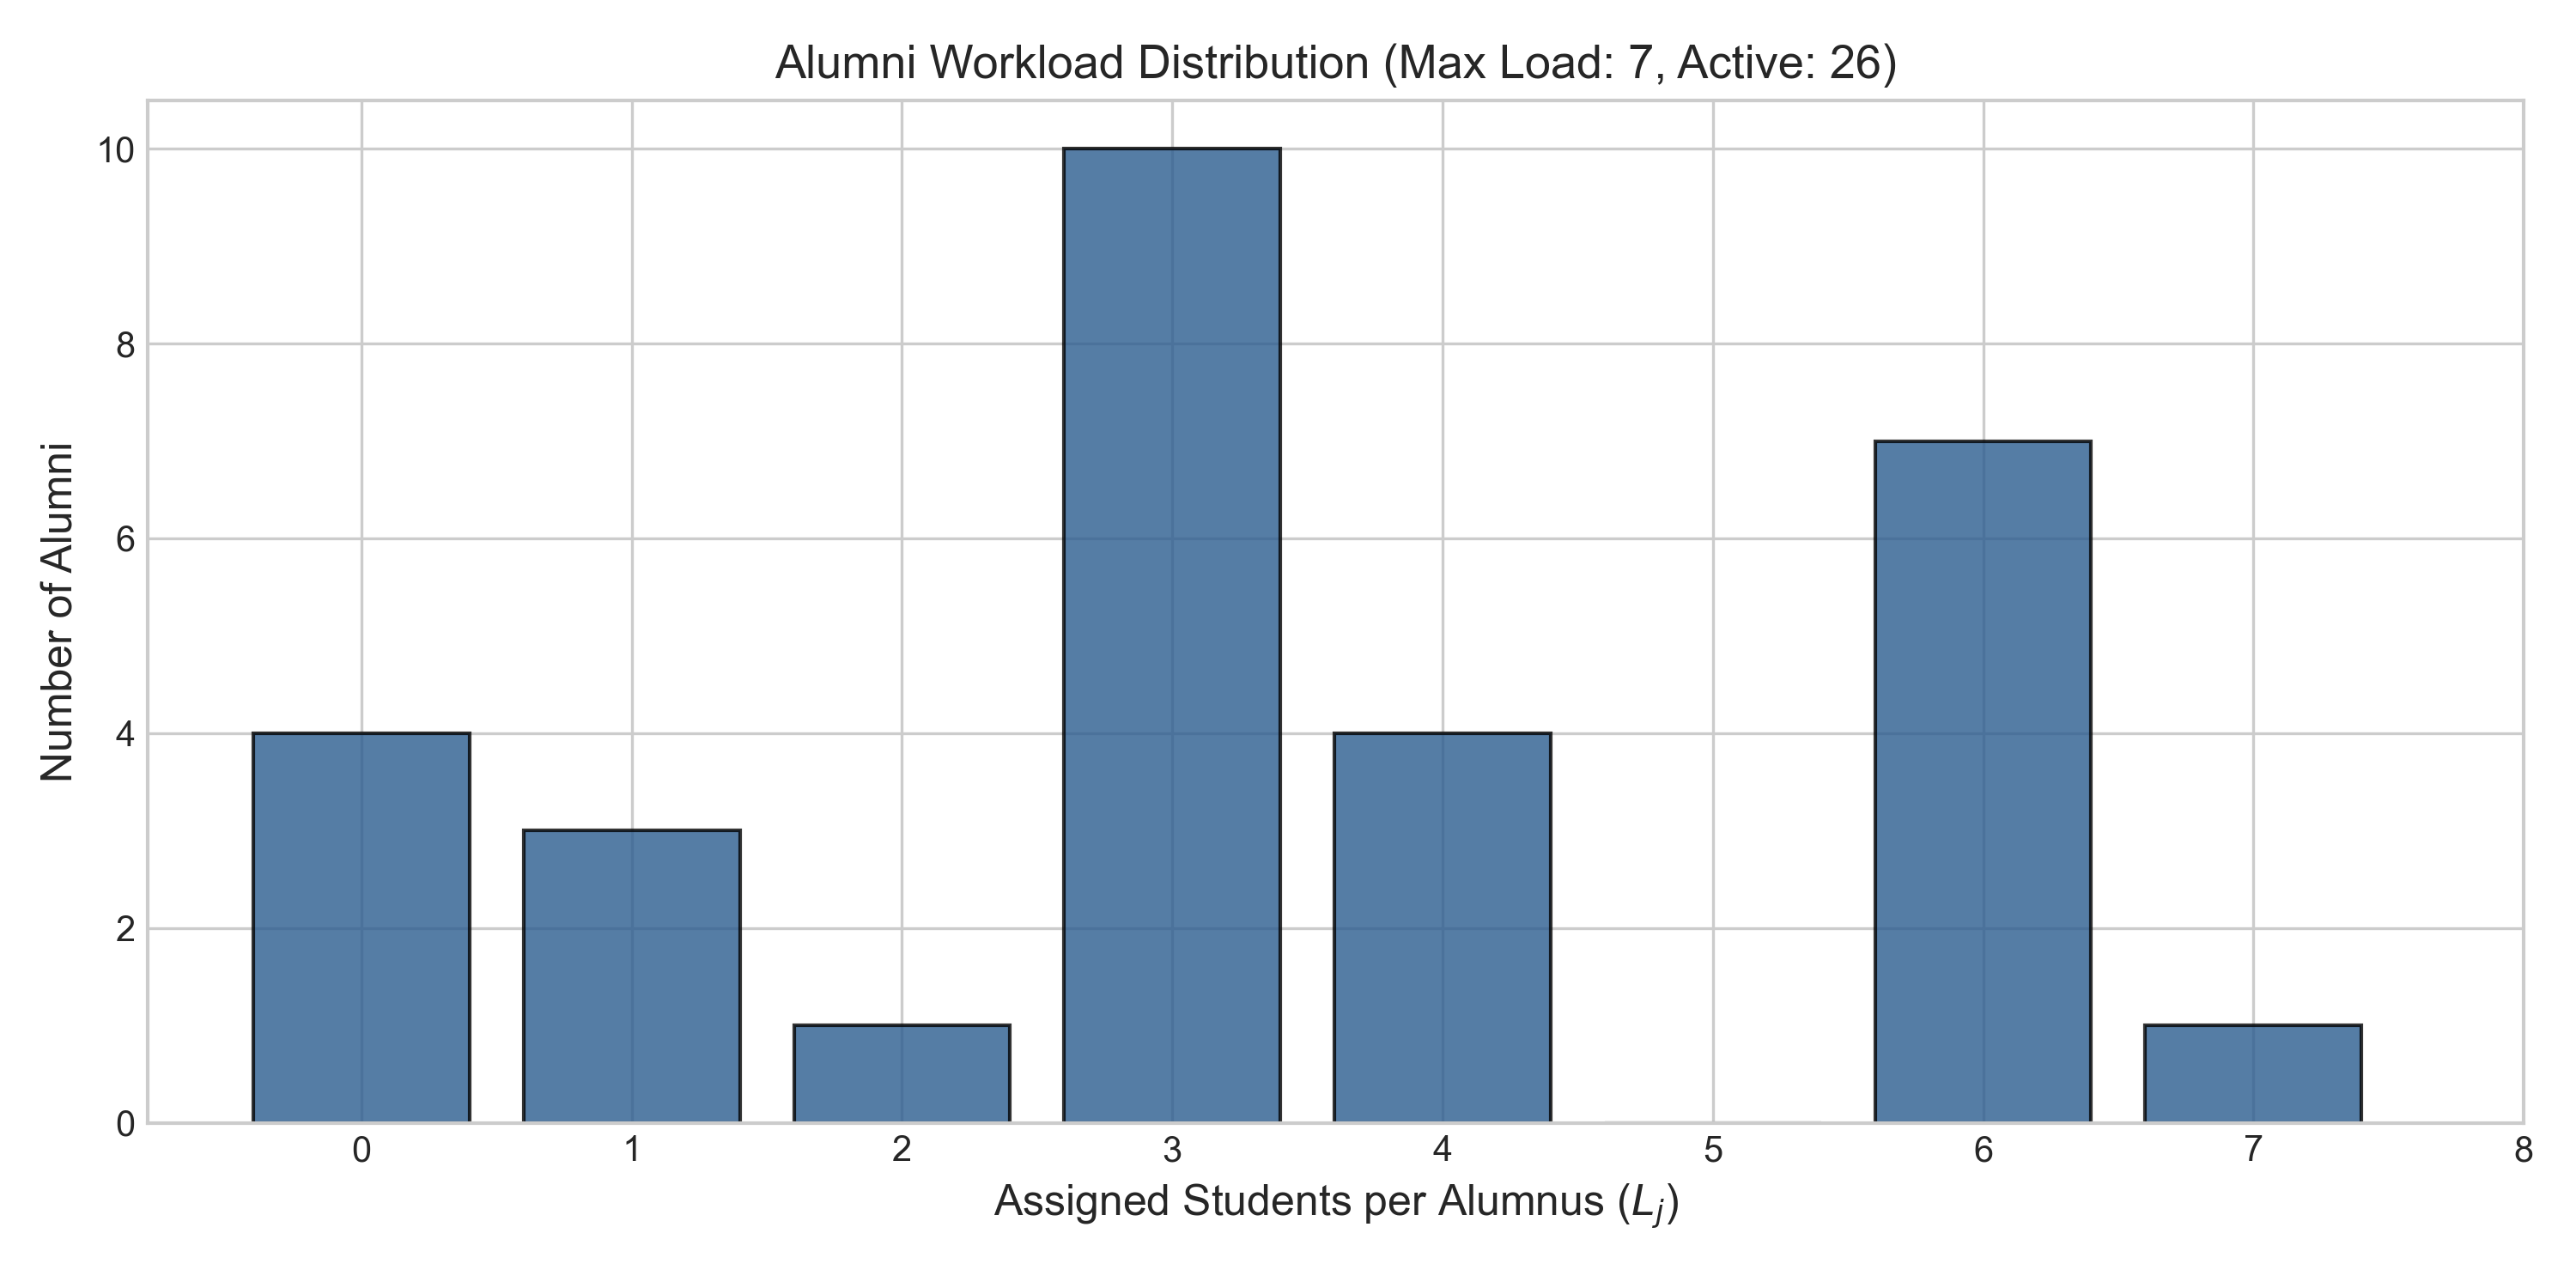
\includegraphics[width=\textwidth]{figures/small_50x30_workload_distribution.png}
    \caption{Alumni workload distribution.}
\end{subfigure}
\caption{Pareto trade-off surface and mentor load compression under the Hybrid Memetic optimizer.}
\label{fig:pareto_workload}
\end{figure}

Figure~\ref{fig:pareto_workload} demonstrates that the Hybrid solver compresses peak mentor load from 8 down to 5.5 while simultaneously elevating worst-student satisfaction from 0.547 to 1.128.

% =============================================================================
% CHAPTER 7: COMPONENT ABLATION & SENSITIVITY
% =============================================================================
\chapter{Component Ablation and Sensitivity Analysis}

\section{Factorial Ablation Study}
To evaluate the contribution of heuristic seeding versus Lamarckian local search, we ran a 30-seed 3-way factorial ablation on \texttt{small\_50x30}.

\begin{table}[htbp]
\centering
\caption{30-seed factorial ablation study results on \texttt{small\_50x30}.}
\label{tab:ablation}
\begin{tabularx}{\textwidth}{lccccc}
\toprule
\textbf{Variant} & \textbf{HV Mean} & \textbf{HV Std} & \textbf{$Z_1$ (Quality)} & \textbf{$Z_2$ (Rawls)} & \textbf{$Z_3$ (Load)} \\
\midrule
Seeding Only & 0.6307 & 0.0641 & 72.62 & 1.095 & 6.00 \\
Local Search Only & 0.3759 & 0.1075 & 66.88 & 1.067 & 5.07 \\
\textbf{Both (Full Hybrid)} & \textbf{0.8704} & \textbf{0.1577} & \textbf{72.64} & \textbf{1.111} & \textbf{5.47} \\
\bottomrule
\end{tabularx}
\end{table}

\begin{figure}[htbp]
\centering
\begin{subfigure}[b]{0.48\textwidth}
    \centering
    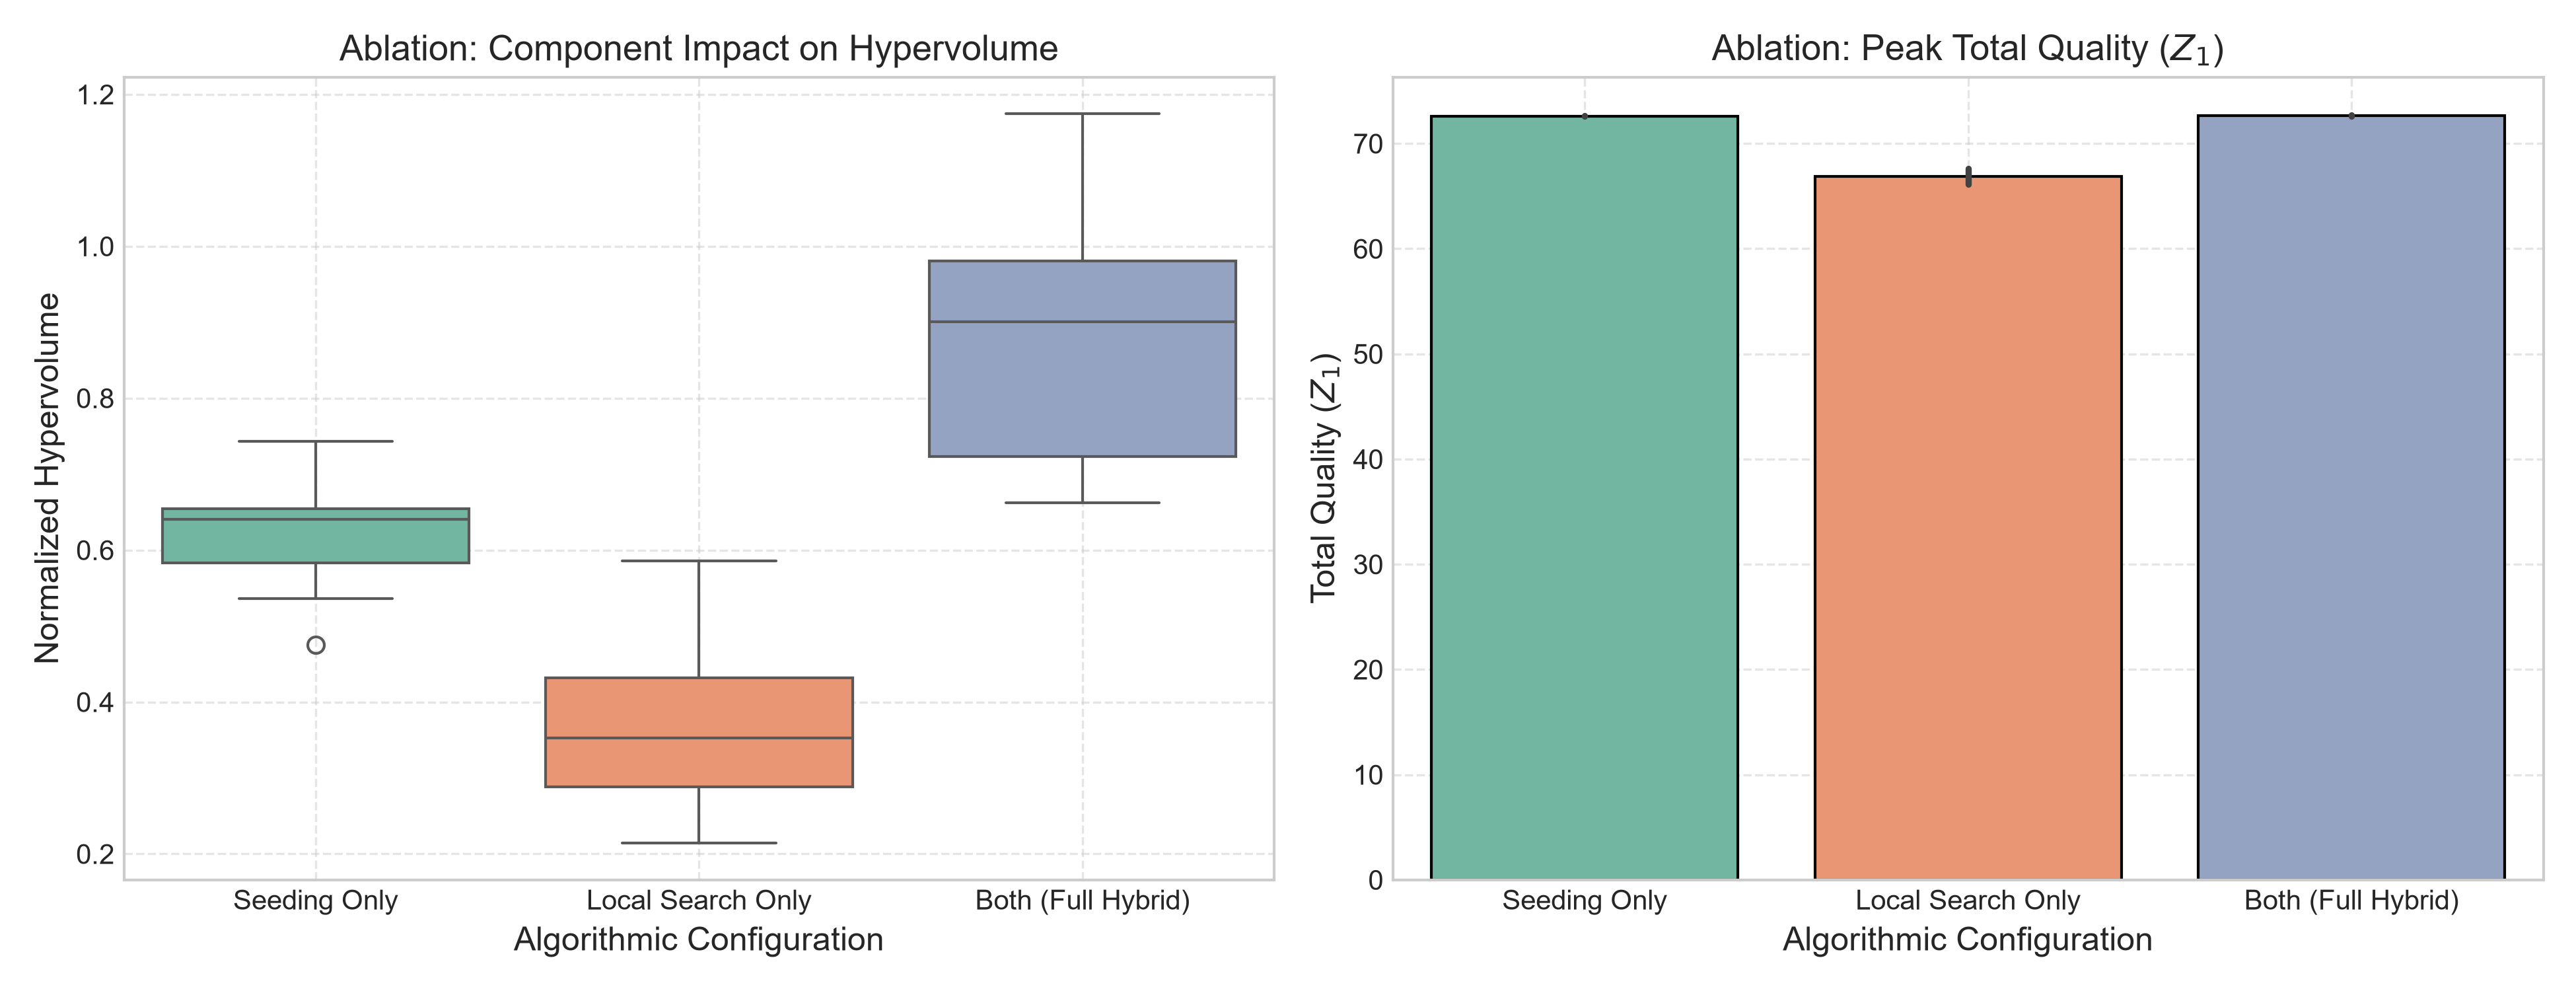
\includegraphics[width=\textwidth]{figures/ablation_study.png}
    \caption{Ablation Hypervolume distributions.}
\end{subfigure}
\hfill
\begin{subfigure}[b]{0.48\textwidth}
    \centering
    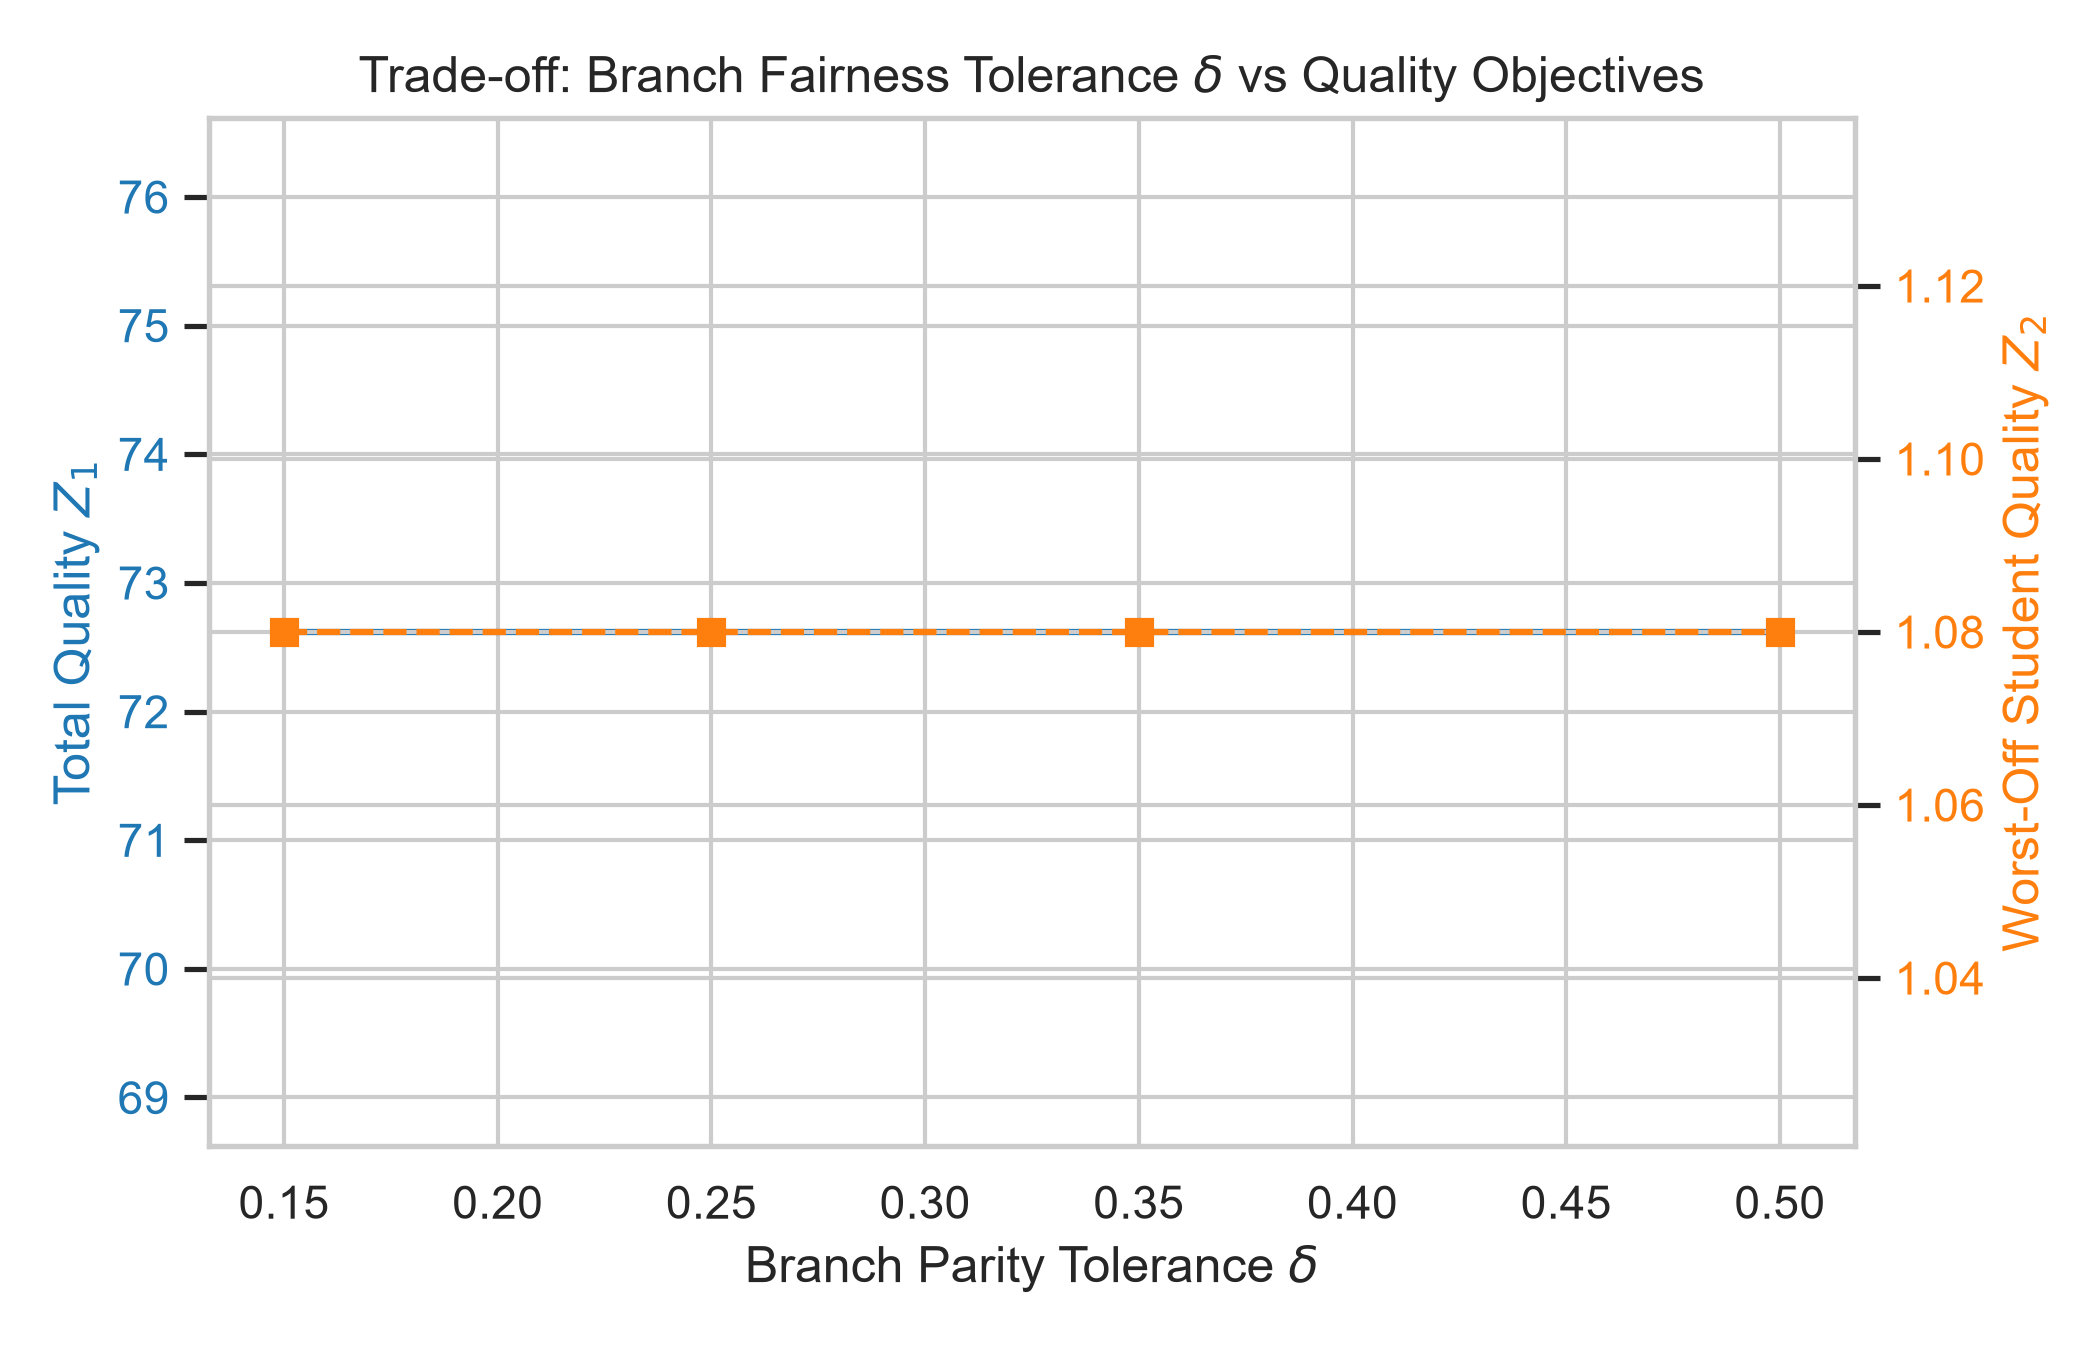
\includegraphics[width=\textwidth]{figures/delta_sensitivity_tradeoff.png}
    \caption{Parity sensitivity sweep ($\delta \in [0.15, 0.50]$).}
\end{subfigure}
\caption{Ablation study distributions and departmental parity sensitivity trade-offs.}
\label{fig:ablation_sensitivity}
\end{figure}

Pairwise Wilcoxon tests confirm that Full Hybrid significantly outperforms Seeding Only ($p = 9.31 \times 10^{-9}, r = 0.987$) and Local Search Only ($p = 1.86 \times 10^{-9}, r = 1.000$), demonstrating super-additive synergy.

% =============================================================================
% CHAPTER 8: THE RECOMMENDATION ROADMAP
% =============================================================================
\chapter{The Recommendation Roadmap}

\section{The Check $\rightarrow$ Improve $\rightarrow$ Measure $\rightarrow$ Decide Framework}
To translate optimization findings into administrative action, institutional initiatives must follow a structured four-stage execution cycle:
\begin{enumerate}
    \item \textbf{Check}: Audit existing departmental registers, consent records, and student domain requests.
    \item \textbf{Improve}: Apply algorithmic matching and targeted 2-opt swaps to eliminate mentor overloading.
    \item \textbf{Measure}: Track realized worst-student quality ($Z_2$), inter-branch disparity ($\delta$), and peak mentor load ($Z_3$).
    \item \textbf{Decide}: Formally ratify mentor allocations and publish individual feedback schedules.
\end{enumerate}

\begin{table}[htbp]
\centering
\caption{Institutional recommendations structured by operational workstream.}
\label{tab:roadmap}
\begin{tabularx}{\textwidth}{lXX}
\toprule
\textbf{Workstream} & \textbf{Primary Operational Focus} & \textbf{Target Metric} \\
\midrule
Workload Balancing & Enforce hard mentor capacity caps ($C_j \le 6$) & Eliminate mentor burnout ($Z_3 \le 6$) \\
Rawlsian Justice & Implement minimum quality floor ($\theta = 0.85 Z_2^{\text{greedy}}$) & Guarantee baseline equity ($Q_i \ge \theta$) \\
Departmental Parity & Restrict inter-branch disparity ($\delta = 1.20 \Delta_{\text{greedy}}$) & Equalize opportunity across branches \\
Corporate Diversity & Limit employer share to $\text{cap}_{\text{comp}} = 1$ & Ensure perspective breadth \\
Continuous Audit & Re-run optimization upon receipt of new alumni registrations & Maintain live Pareto frontier \\
\bottomrule
\end{tabularx}
\end{table}

% =============================================================================
% CHAPTER 9: SOFTWARE ARCHITECTURE AND LIVE DEMO UI
% =============================================================================
\chapter{Software Architecture and Live Demo UI}

\section{Repository Architecture}
The project codebase is organized into five modular tiers:
\begin{itemize}
    \item \textbf{Data Tier} (\texttt{src/data\_generator.py}): Parametric instance synthesis with log-normal capacities.
    \item \textbf{Problem Tier} (\texttt{src/problem.py}): Vector evaluation and calibration functions.
    \item \textbf{Algorithms Tier} (\texttt{src/algorithms/}, \texttt{src/hybrid/}): NSGA-II, SPEA2, MOEA/D, and Hybrid.
    \item \textbf{Metrics Tier} (\texttt{src/metrics.py}): Shared reference Hypervolume, Gini, and Wilcoxon tests.
    \item \textbf{Presentation Tier} (\texttt{ui\_demo.py}): Interactive Streamlit dashboard.
\end{itemize}

\section{Interactive Decision-Support UI}
To facilitate live stakeholder demonstrations, we created \texttt{ui\_demo.py}. Running \texttt{streamlit run ui_demo.py} launches a web-based dashboard allowing administrators to select instance sizes, calibrate $\theta$ and $\delta$, execute benchmarks, and inspect Pareto surfaces in real time.

% =============================================================================
% CHAPTER 10: LIMITATIONS AND FUTURE SCOPE
% =============================================================================
\chapter{Limitations and Future Scope}

\section{Limitations}
\begin{itemize}
    \item Synthetic data environment necessitated by student privacy mandates.
    \item Static compatibility model assuming deterministic preferences.
    \item Exact MILP branch-and-cut restricted to small cohorts ($50 \times 30$).
\end{itemize}

\section{Future Scope}
\begin{itemize}
    \item Integration of Gale-Shapley two-sided stability constraints.
    \item Chance-constrained stochastic programming to model mentor availability risk.
    \item Departmental pilot deployment at VJTI with longitudinal feedback auditing.
\end{itemize}

% =============================================================================
% CHAPTER 11: CONCLUSION & GUIDANCE
% =============================================================================
\chapter{Conclusion and Strategic Guidance}

\section{Conclusion}
This project formulated, solved, and benchmarked the Multi-Objective Capacitated Bipartite Assignment Problem for VJTI Mumbai. The engineered \textbf{Hybrid Seeded Memetic NSGA-II} algorithm achieved an 8-fold hypervolume advantage over standard baselines, strictly dominated Greedy matching in 100\% of seeds, and reduced mentor burnout while elevating worst-student satisfaction.

\section{Strategic Guidance for Institutional Leadership}
\begin{enumerate}
    \item \textbf{Abolish First-Come-First-Served Allocations}: Greedy matching predictably induces mentor burnout and student neglect.
    \item \textbf{Select from the Pareto Frontier}: Use multi-objective trade-offs to select balanced assignments.
    \item \textbf{Deploy Data-Driven Calibration}: Calibrate $\theta$ and $\delta$ dynamically from empirical baseline distributions.
    \item \textbf{Embed Continuous Auditing}: Incorporate the interactive Streamlit dashboard into annual placement operations.
\end{enumerate}

\vspace{1.0cm}
\begin{center}
\textit{``Optimizing institutional performance through intelligent resource allocation.''}
\end{center}

% =============================================================================
% REFERENCES
% =============================================================================
\newpage
\begin{thebibliography}{99}
\bibitem{deb2002fast}
K.~Deb, A.~Pratap, S.~Agarwal, and T.~Meyarivan.
\newblock A fast and elitist multiobjective genetic algorithm: {NSGA-II}.
\newblock {\em IEEE Transactions on Evolutionary Computation}, 6(2):182--197, 2002.

\bibitem{zitzler2001spea2}
E.~Zitzler, M.~Laumanns, and L.~Thiele.
\newblock {SPEA2}: Improving the strength {Pareto} evolutionary algorithm.
\newblock {\em TIK-Report}, 103, 2001.

\bibitem{zhang2007moea}
Q.~Zhang and H.~Li.
\newblock {MOEA/D}: A multiobjective evolutionary algorithm based on decomposition.
\newblock {\em IEEE Transactions on Evolutionary Computation}, 11(6):712--731, 2007.

\bibitem{gale1962college}
D.~Gale and L.~S. Shapley.
\newblock College admissions and the stability of marriage.
\newblock {\em The American Mathematical Monthly}, 69(1):9--15, 1962.

\bibitem{rawls1971theory}
J.~Rawls.
\newblock {\em A Theory of Justice}.
\newblock Harvard University Press, 1971.

\bibitem{huang2021highs}
Q.~Huangfu and J.~A.~J. Hall.
\newblock {HiGHS}: High performance software for linear optimization.
\newblock {\em Mathematical Programming Computation}, 10(2):119--142, 2018.

\bibitem{blank2020pymoo}
J.~Blank and K.~Deb.
\newblock {pymoo}: Multi-objective optimization in {Python}.
\newblock {\em IEEE Access}, 8:89497--89509, 2020.

\bibitem{ahuja1993network}
R.~K. Ahuja, T.~L. Magnanti, and J.~B. Orlin.
\newblock {\em Network Flows: Theory, Algorithms, and Applications}.
\newblock Prentice Hall, 1993.
\end{thebibliography}

% =============================================================================
% APPENDIX A: TEAM CONTRIBUTIONS
% =============================================================================
\chapter{Team Contributions}
\begin{table}[htbp]
\centering
\caption{Division of work among project team members.}
\label{tab:division_of_work}
\begin{tabularx}{\textwidth}{llll}
\toprule
\textbf{Member} & \textbf{Roll No.} & \textbf{Workstream} & \textbf{Principal Contributions} \\
\midrule
Utkarsh Gupta & 241070078 & System Formulation Lead & MO-CBAP modeling, report assembly, threshold calibration \\
Aryan Doshi & 241070022 & Evolutionary Algorithms Lead & NSGA-II, SPEA2, MOEA/D implementation and 30-seed runs \\
Indraneel Hajarnis & 241070025 & Memetic Lead & 2-opt local search moves, elitist archiving, Streamlit UI \\
Dhairya Dabi & 241070015 & Baseline \& Sensitivity Lead & HiGHS MILP, MCF repair operator, Wilcoxon testing \\
\bottomrule
\end{tabularx}
\end{table}

% =============================================================================
% APPENDIX B: GLOSSARY OF ABBREVIATIONS
% =============================================================================
\chapter{Glossary of Abbreviations}
\begin{table}[htbp]
\centering
\caption{Abbreviations used throughout this report.}
\label{tab:abbreviations}
\begin{tabularx}{\textwidth}{llX}
\toprule
\textbf{Term} & \textbf{Category} & \textbf{Meaning / Definition} \\
\midrule
MO-CBAP & Optimization & Multi-Objective Capacitated Bipartite Assignment Problem \\
NSGA-II & Meta-Heuristic & Non-dominated Sorting Genetic Algorithm II \\
SPEA2 & Meta-Heuristic & Strength Pareto Evolutionary Algorithm 2 \\
MOEA/D & Meta-Heuristic & Multiobjective Evolutionary Algorithm based on Decomposition \\
MILP & Exact Solver & Mixed-Integer Linear Programming \\
MCF & Baseline & Minimum-Cost Flow \\
HV & Metric & Hypervolume \\
VJTI & Institution & Veermata Jijabai Technological Institute, Mumbai \\
CE / IT & Departments & Computer Engineering / Information Technology \\
EXTC / EE & Departments & Electronics \& Telecomm. / Electrical Engineering \\
ME / CEV & Departments & Mechanical / Civil and Environmental Engineering \\
PE / TT & Departments & Production Engineering / Textile Technology \\
\bottomrule
\end{tabularx}
\end{table}

\end{document}
